%!TEX root = kotov.tex
\section{Task 1: Префиксы префиксов}
\begin{task}
    Для каждого префикса строки найти количество его префиксов, равных его суффиксу $\O(n)$.
\end{task}

\begin{solution}
    Ох опять промазал :)

    Рассмотрим подстроку, соответствующая наибольшему значению в префикс-функции:
    \begin{figure}[H]
        \centering
        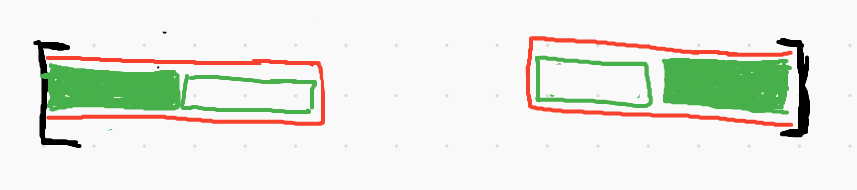
\includegraphics[width=0.4\textwidth]{pics/1.png}
        \caption{Подстрока с наибольшим значением префикс-функции.}
    \end{figure}
    На этом рисунке черным обозначен как раз такой префик, у которого длина совпадающего префикса с суффиксом наибольшая (ох какая сложная семантика) среди всех префиксов исходной строки. Красным обозначены как раз соответствующие совпадающие кусочки.

    Теперь заметим, что закрашенный зеленый кусочек --- префикс красной, причем такой, что у него есть парный суффикс, т. е. в правом красном справа есть еще такой же закрашенный зеленый кусочек. Заметим далее, что так как левый красный равен правому красному, то правый закрашенный равен незакрашенному зеленому в левом красном, что даст еще один префикс, у которого будет нужное свойство.

    Пусть $\pi[i]$ --- префиксная функция. Заведем массив $d[i]$ --- количество совпадений в соответствующих префиксах, тогда можно посчитать $d[i] = 1 + d[\pi[i]]$, т.е. получилась такая некая динамика, причем пройдемся мы один раз по всему массиву, ну и, видимо, для чистоты стоит сказать, что в крайнем самом левом случае положить $d$ равным $1$.

    \begin{remark}
        Вроде как, если похитрить, то можно посчитывать $d$ в процессе обхода слева-направо, пока мы считаем префиксную функцию, тогда явно будет $\O(n)$
    \end{remark}
\end{solution}